\documentclass[tikz]{standalone}%

\usepackage[utf8]{inputenx}%  http://ctan.org/pkg/inputenx
% Euler for math | Palatino for rm | Helvetica for ss | Courier for tt
\renewcommand{\rmdefault}{ppl}% rm
\linespread{1.05}% Palatino needs more leading
\usepackage[scaled]{helvet}% ss //  http://ctan.org/pkg/helvet
\usepackage{courier}% tt // http://ctan.org/pkg/courier
\usepackage{eulervm}  %  http://ctan.org/pkg/eulervm
% a better implementation of the euler package (not in gwTeX)
\normalfont%
\usepackage[T1]{fontenc}%  http://ctan.org/pkg/fontenc
\usepackage{textcomp}%  http://ctan.org/pkg/textcomp

\usetikzlibrary{calc}
\usetikzlibrary{intersections}
\usetikzlibrary{angles}
\usetikzlibrary{quotes}
\usetikzlibrary{decorations.markings}

\begin{document}
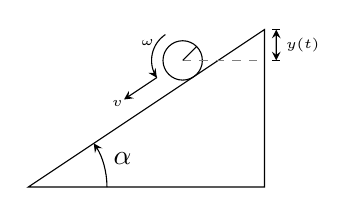
\begin{tikzpicture}
  \coordinate (A) at (0, 0);
  \coordinate (B) at (3, 0);
  \coordinate (C) at (3, 2);

  \draw[name path = tri] (A) -- (B) -- (C) -- cycle pic["$\alpha$", -stealth,
  draw, angle radius = 1cm, angle eccentricity = 1.25] {angle = B--A--C};

  \path[name path = line] (0, 1.4) -- +(2.9, 0);
  \path[name intersections = {of = line and tri, by = P1}];
  \path (P1) -- ($(P1)!.25cm!-90:(A)$) coordinate (cylinder);
  \path[name path = line2] (cylinder) -- +(1.05, 0);
  \path[name intersections = {of = line2 and tri}];

  \draw (cylinder) circle[radius = 0.25cm];
  \draw[dashed, gray] (cylinder) -- (intersection-1);
  \draw[stealth-stealth] (3.15, 2) -- ($(intersection-1) + (.15, 0)$)
  node[pos = .5, right, font = \tiny] {$y(t)$};
  \draw (3.1, 2) -- (3.2, 2);
  \draw ($(intersection-1) + (.1, 0)$) -- +(.1, 0);
  \draw (cylinder) -- +(45:.25);

  \pgfmathsetmacro{\angle}{atan(2/3)};
  \pgfmathsetmacro{\ppi}{\angle + 180};
  
  \begin{scope}[rotate = \angle, decoration = {
      markings,
      mark = at position 0.5 with {\arrow{stealth}}
    }]
    \clip ($(cylinder) + (0, .5)$) rectangle ($(cylinder) + (-.45, 0)$);

    \draw[name path global = rotation, postaction = decorate] (cylinder)
    circle[radius = .395cm] node[font = \tiny] at +(120:.5) {$\omega$};
  \end{scope}

  \path[name path = line3] (cylinder) -- +(\ppi:.4);
  \path[name intersections = {of = line3 and rotation, by = P2}];

  \draw[-stealth] (P2) -- ++(\ppi:.5) node[font = \tiny, pos = 1.2] {$v$};
\end{tikzpicture}
\end{document}
%%% Local Variables:
%%% mode: latex
%%% TeX-master: t
%%% End:
